% unicodeは、hyperrefへの指定で、pdfのメタデータにあるタイトルの文字化けを防ぐ
% ptは細かい指定はできないらしい
% チートシート
% https://www.cpt.univ-mrs.fr/~masson/latex/Beamer-appearance-cheat-sheet.pdf
\documentclass[unicode, 14pt, aspectratio=169]{beamer} 
\usepackage{minted}
\usepackage{listings}
\usepackage{enumitem}
\usepackage{xcolor}
\usepackage{textcomp}
\usepackage[backend=biber, style=ieee]{biblatex}
\usetheme{rikako}
\date{\number\year 年\number\month 月\number\day 日}
\addbibresource{main.bib}
\title{runcのUNIXプログラミング}
\author{\texttt{ryotaro612}}
\begin{document}
\usemintedstyle{titech}
\begin{frame}[noframenumbering, plain]
\titlepage
\end{frame}
\section{導入}
\begin{frame}[t]
  \frametitle{runc}
  \large
  低レベルなコンテナランタイムのCLI
  \normalsize
  \begin{figure}
    \centering
    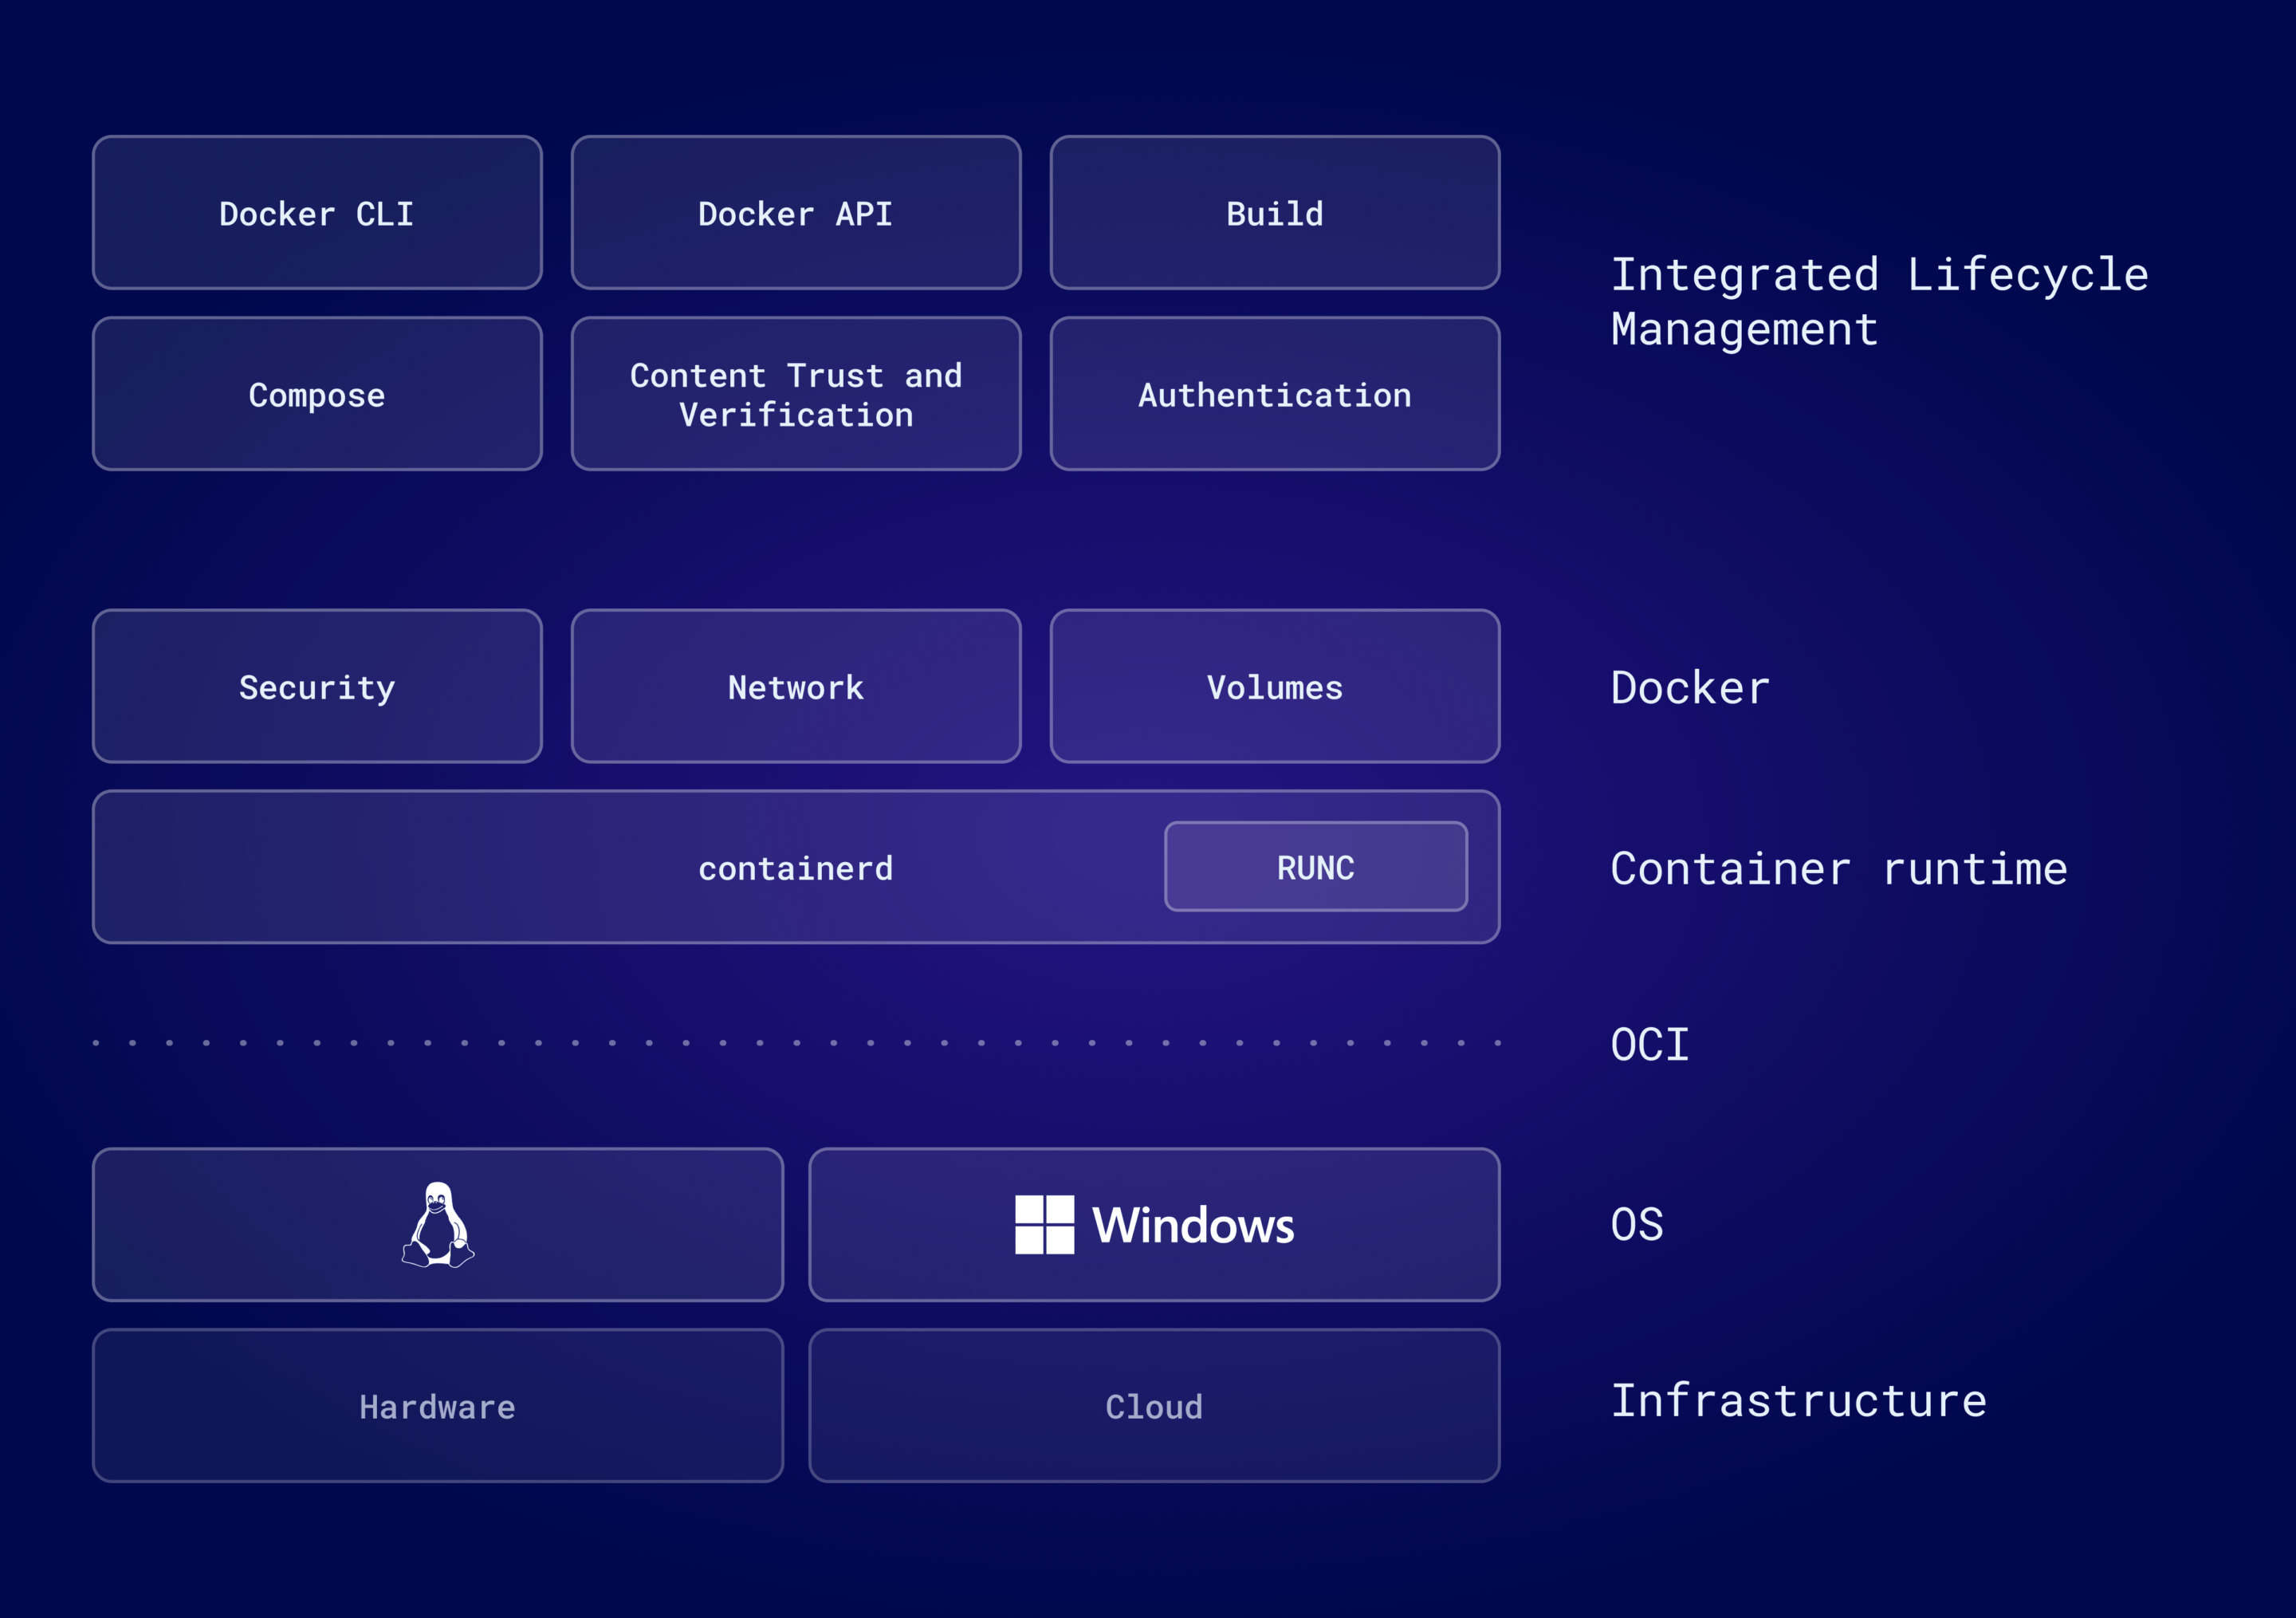
\includegraphics[width=6.2cm]{images/containerd-diagram-v1.png} 
    \caption{Docker, runc, OSの階層\footnote{\scriptsize{\href{https://www.docker.com/blog/containerd-vs-docker}{containerd vs. Docker: Understanding Their Relationship and How They Work Together}より}}}
    \label{fig:runc}
  \end{figure}
\end{frame}
\begin{frame}[t]%[fragile=singleslide]
  \frametitle{抽象度の低い\texttt{runc}}
  \large
  イメージは不要、コンテナのルート\texttt{/}で十分
  \normalsize
  \begin{center}
    \inputminted[fontsize=\small]{sh}{code/run.sh}
    runcでコンテナの\texttt{sh}を開始
  \end{center}
\end{frame}
\begin{frame}[t]
  \frametitle{資料の目的}
  \large
  UNIXプログラミングの基本的な道具を知る
  \normalsize 
  \begin{center}
    Infrastructure Plumbing Manifesto\footnote{\scriptsize{dockerのブログ \href{https://www.docker.com/blog/runc/}{Introducing runC: a lightweight universal container runtime
}より}}
    \end{center}
  \begin{quote}
    \begin{itemize}
    \item {\small When you need to create new plumbing, make it easy to re-use and contribute improvements back.}
    \item {\small Follow the unix principles: several simple components are better than a single, complicated one.}
    \item {\small Define standard interfaces which can be used to combine many simple components into a more sophisticated system.}
  \end{itemize}
\end{quote}
  runcはUNIXの原則による小さな機能を組合せ
\end{frame}
\begin{frame}[t]
  \frametitle{runc runの手続き}
  \large
  \texttt{run}の呼出す\texttt{init}がコンテナになる
  \normalsize
  % \texttt{run}の呼出す\texttt{init}が\href{https://man7.org/linux/man-pages/man2/execve.2.html}{execve}でコンテナのプロセスになる
  \begin{figure}
    \centering
    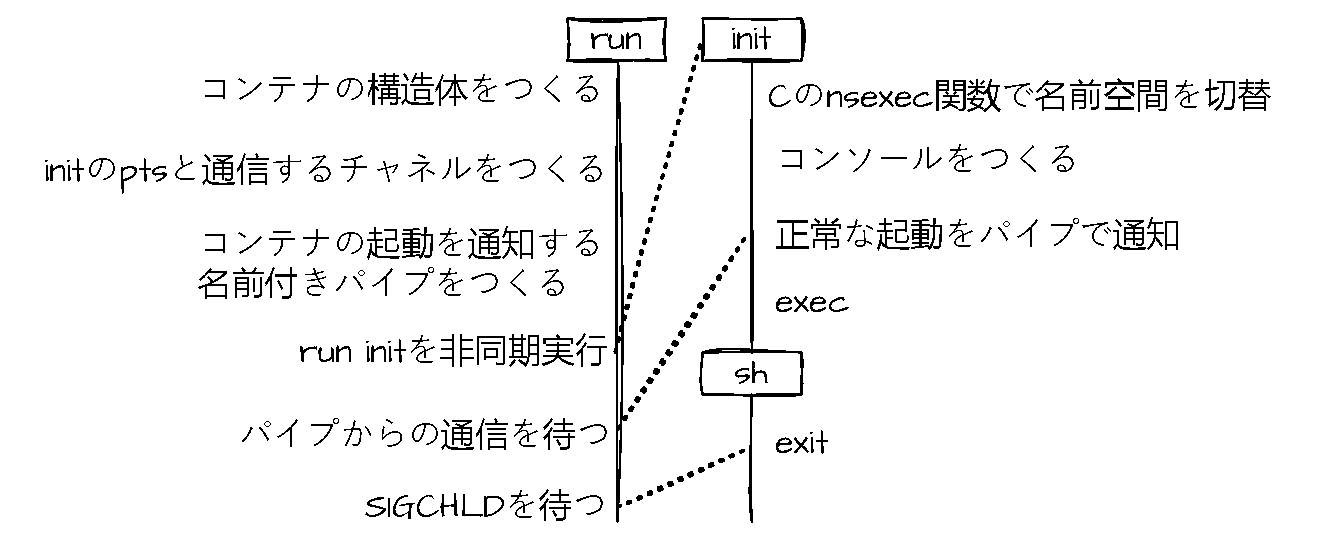
\includegraphics[width=13cm]{images/overview.drawio.pdf}
    \caption{runとinitコマンドの手続き} %\footnote{点線はプロセスを横断する処理}
  \end{figure}
  \texttt{init}はコンテナのPID 1のプロセスになる
\end{frame}
\section{ホストとコンテナの端末間通信}
\begin{frame}[t]
  \frametitle{疑似端末 \texttt{pty}}
  \large
  \texttt{pty}はキャラクタデバイスのマスタ、スレーブの組\supercite{pty}
  \normalsize
  \begin{itemize}[leftmargin=0.8cm,label=$\circ$]
  \item マスタ\texttt{/dev/ptmx}を開くと\texttt{/dev/pts}下にスレーブができる
  \item 一方の入力が他方の出力になる
  \item \href{https://man7.org/linux/man-pages/man3/ptsname.3.html}{\texttt{ptsname}}関数にマスタのファイル記述子を渡すとスレーブのパスがわかる
  \item 通常、プロセスはマスタを開いてforkする。子プロセスはスレーブを複製して標準I/O, エラーにする\supercite{advancedunix}\footnote{\texttt{ls -l /proc/<pid>/fd}で記述子0, 1, 2がスレーブへのリンクか分かる}
  \end{itemize}
\end{frame}
\begin{frame}[t]
  \frametitle{\texttt{runc}での\texttt{pty}の準備}
  \large
  \texttt{init}は\texttt{run}にマスタのファイル記述子を送る\footnote{\scriptsize{次ページより上の手続きの実装を確認する}}
  \normalsize
  \setlist[enumerate]{label*=\arabic*.,ref=\arabic*}
  \begin{enumerate}[leftmargin=1.2cm]
  \item \texttt{run}は\href{https://man7.org/linux/man-pages/man2/socketpair.2.html}{\texttt{socketpair}}でソケットの組をつくる。双方向通信できる
  \item \texttt{run}は\href{https://pkg.go.dev/os/exec\#Cmd}{\texttt{Cmd.ExtraFiles}}でソケットを1つ\texttt{init}にわたす
  \item \texttt{init}は\texttt{/dev/ptmx}を開く
  \item \texttt{init}は\href{https://man7.org/linux/man-pages/man3/sendmsg.3p.html}{sendmsg}でソケットを通してマスタを\texttt{run}に送る
  \item \texttt{run}はマスタの入出力を標準IOにコピーする
  \end{enumerate}
\end{frame}
\begin{frame}[t]
  \frametitle{\texttt{init}}
  \large
  マスタを開き、その記述子を\texttt{run}に送る
  \normalsize
  \begin{center}
    \inputminted{go}{code/tty_init.go}
    \href{https://github.com/opencontainers/runc/blob/7cb363254b69e10320360b63fb73e0ffb5da7bf2/libcontainer/init_linux.go\#L371}{\texttt{setupConsole}}関数の抜粋
  \end{center}
\end{frame}
\begin{frame}[t]
  \frametitle{\texttt{init}}
  \large
  \href{https://ja.manpages.org/dup3/2}{dup3}でスレーブを複製
  \normalsize
  \begin{center}
    \inputminted{go}{code/pty_init_dup.go}
    \href{https://github.com/opencontainers/runc/blob/7cb363254b69e10320360b63fb73e0ffb5da7bf2/libcontainer/console_linux.go\#L28}{\texttt{dupStdio}}関数の抜粋
  \end{center}
  コードの\texttt{0, 1, 2}は標準IO, エラー出力の記述子
\end{frame}
\begin{frame}[t]
  \frametitle{\texttt{init}}
  \large
  スレーブをプロセスの制御端末にする\supercite{ioctl}
  \normalsize
  \begin{center}
    \inputminted{go}{code/pty_tty.go}
    \href{https://github.com/opencontainers/runc/blob/7cb363254b69e10320360b63fb73e0ffb5da7bf2/libcontainer/system/linux.go\#L121}{\texttt{Setctty}}関数の抜粋
  \end{center}
\end{frame}
\begin{frame}[t]
  \frametitle{\texttt{run}}
  \large
  ホストの標準入力をマスタに書き、マスタの出力を\\ホストの標準出力に送る  
  \normalsize
  \begin{center}
    \small{\inputminted{go}{code/tty_run.go}}
    \href{https://github.com/opencontainers/runc/blob/7cb363254b69e10320360b63fb73e0ffb5da7bf2/tty.go\#L102}{\texttt{recvtty}}関数の抜粋
  \end{center}
  \href{https://man7.org/linux/man-pages/man7/epoll.7.html}{\texttt{epoll}}でマスタの入出力を監視
\end{frame}
\section{名前空間}
\begin{frame}[t]
  \frametitle{名前空間\supercite{namespaces}}
  \large
  空間のプロセスには自分達がリソースを占有したように見える
  \normalsize 
  \begin{itemize}[leftmargin=0.8cm,label=$\circ$]
    \item マウントポイント、プロセスIDなど6種類の名前空間がある
    \item 名前空間の間でリソース名が重複しても互いに影響しない
    \item API
      \begin{description}[leftmargin=4.8em,style=nextline]
      \item[\href{https://man7.org/linux/man-pages/man2/clone.2.html}{\texttt{clone}}] 新しいプロセスを作る。子プロセスを新しい名前空間に入れることもできる
      \item[\href{https://man7.org/linux/man-pages/man2/setns.2.html}{\texttt{setns}}] 呼びだしたスレッドを既存の名前空間に入れる。用途はコンテナ間でのネットワークの共有など
      \item[\href{https://man7.org/linux/man-pages/man2/unshare.2.html}{\texttt{unshare}}] 指定した種類の名前空間を作り、呼びだしたプロセスを移動する
      \end{description}
    \end{itemize}
\end{frame}
\begin{frame}[t]
  \frametitle{\texttt{nsexec}で\texttt{init}の名前空間を移動}
  \large
  Goの前にCの\texttt{nsexec}関数を実行する
  \normalsize
  \begin{center}
    \inputminted{go}{code/nsenter.go}
    \href{https://github.com/opencontainers/runc/blob/7cb363254b69e10320360b63fb73e0ffb5da7bf2/libcontainer/nsenter/nsenter.go\#L12}{\texttt{nsenter.go}}の抜粋
  \end{center}
  Goのランタイムには複数のスレッドがあるが、\texttt{setns}は呼びだしたスレッドの名前空間のみを移動する\supercite{runc}
\end{frame}
\begin{frame}[t]
  \frametitle{\texttt{nsexec}}
  \large
  \texttt{clone}でpid 1を割り当てる
  \normalsize
  \begin{columns}
    \begin{column}{0.5\textwidth}
      \begin{itemize}[leftmargin=0.8cm,label=$\circ$]
      \item \href{https://man7.org/linux/man-pages/man2/clone.2.html}{\texttt{clone}}に\texttt{CLONE\_PARENT}を渡すことで、新しい\texttt{init}の親プロセスを常に\texttt{run}にし、\texttt{SIGCHLD}を\texttt{run}に届ける
      \item \texttt{uid\_map}, \texttt{gid\_map}には、親と子の名前空間のユーザ、グループIDの写像を書く\supercite{usernamespaces}
      \end{itemize}
    \end{column}
    \begin{column}{0.5\textwidth}
      \begin{figure}
        \centering
        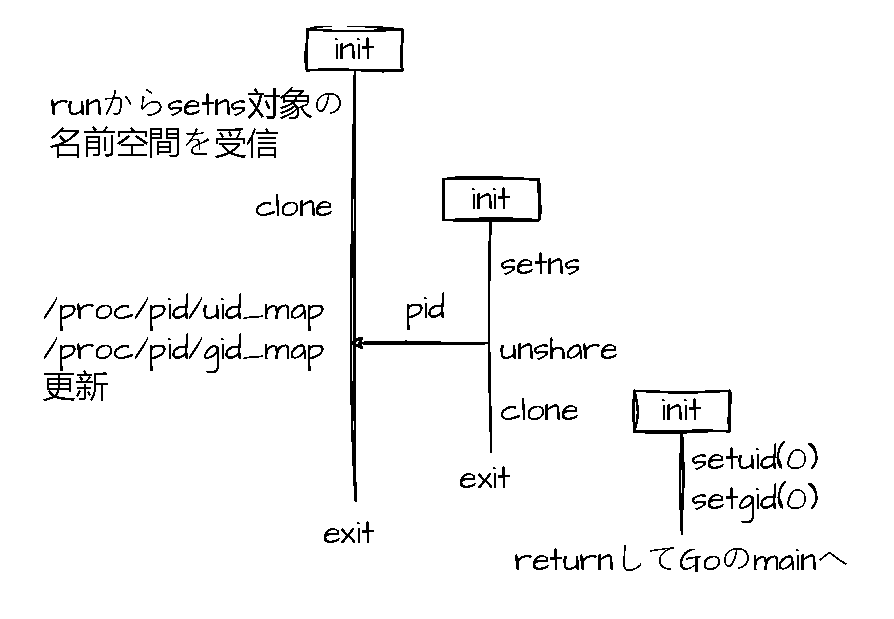
\includegraphics[width=5.5cm]{images/nsenter.drawio.pdf}
        \caption{\texttt{nsexec}の処理手順}
        \label{fig:nsenter}
      \end{figure}      
    \end{column}
  \end{columns}
  \texttt{unshare}では呼出元のプロセス名前空間を変更できない\supercite{unshare}
\end{frame} 
\section{ファイルシステムの変更}
\begin{frame}[t]
  \frametitle{\texttt{init}のルートファイルシステムを変更}
  \large
  \href{https://man7.org/linux/man-pages/man2/pivot_root.2.html}{\texttt{pivot\_root}}でファイルシステムを変更する
  \normalsize
  \begin{center}
    \inputminted{sh}{code/pivot_root.sh}
    \texttt{pivot\_root}の実行例
  \end{center}
\end{frame}
\section{伝えたかったこと}
\begin{frame}[t]
  \frametitle{実装とPlumbling Manifestoをふりかえって}
  \large
  コンテナの基礎の実装に特別なからくりはない
  \normalsize
  \begin{itemize}[leftmargin=0.8cm,label=$\circ$]
  \item 標準のインターフェース
    \begin{itemize}[leftmargin=0.8cm,label=$\circ$]
    \item 端末, 名前空間、マウントは互いに異質だが、どれも\texttt{/proc}下のディレクトリ(\texttt{ns}, \texttt{fd}, \texttt{mounts})にファイルとして、その状態が公開されている
    \item ファイル開き、返った記述子を関数に渡して操作できる
    \end{itemize}
  \item 小さな機能の組合せ
    \begin{itemize}[leftmargin=0.8cm,label=$\circ$]
      \item コンテナに用途を限らない機能で実装されている
        \footnote{\texttt{clone}の\texttt{CLONE\_NEWIPC}などコンテナのために用意された機能も一部ある\supercite{clone}}
      \item \texttt{runc}自体も抽象度の高いAPIから組合せられて使われる
    \end{itemize}
  \end{itemize}  
\end{frame}

% \section{付録 コンテナの構造体}
% \begin{frame}
%   \frametitle{libcontainer.Container}
%   フィールドは非公開
%   \begin{columns}
%     \begin{column}{0.5\textwidth}
%       \begin{center}
%         \inputminted{go}{code/container.go}
%         libcontainer.Container\supercite{libcontainer}
%       \end{center}
%     \end{column}
%     \begin{column}{0.5\textwidth}
%       \begin{itemize}[leftmargin=0.2cm,label=$\circ$]
%         \item \texttt{stateDir}は\texttt{runc}の\texttt{--root}オプション\texttt{<dir>}とすると\texttt{<dir>/<id>}
%         \item \texttt{stateDir}には\texttt{run init}を呼びだす \texttt{/proc/self/exe}の複製や名前つきパイプをおく
%         \item \texttt{/proc/self/exe}は実行中のプログラムのパスのシンボリックリンク
%       \end{itemize}
%     \end{column}
%   \end{columns}
% \end{frame}
% \begin{frame}
%   プロセスの非機能を隔離、監視\supercite{rdt}する
%   \frametitle{libcontainer.Container}
%   \begin{center}
%     \inputminted{go}{code/container2.go}
%     libcontainer.Container\supercite{libcontainer}
%   \end{center}
% \end{frame}
% \begin{frame}
%   コンテナで実行したいプロセスの情報がある
%   \frametitle{libcontainer.Container}
%   \begin{center}
%     \inputminted{go}{code/container3.go}
%     libcontainer.Container\supercite{libcontainer}
%   \end{center}
% \end{frame}
% \begin{frame}[t]
%   \frametitle{libcontainer.Container}
%   コンテナのチェックポイント、リストアのフィールドがある\supercite{criu}
%   \begin{center}
%     \inputminted{go}{code/container4.go}
%     libcontainer.Container\supercite{libcontainer}
%   \end{center}
% \end{frame}
\begin{frame}[allowframebreaks]
  \frametitle{参考資料}
  \printbibliography
  \nocite{*}
\end{frame}
\end{document}
